\subsection*{Dane eksperymentu}
Liczba punktów $m=5$; znane ograniczenie górne na minimalny stopień: $(m-1)^2=16$.
\begin{center}\begin{tabular}{ccc}\toprule $i$ & $p_i$ & $q_i$\\\midrule
1 & $(-1,\ -1)$ & $(1,\ 1)$\\
2 & $(1,\ -1)$ & $(-1,\ 1)$\\
3 & $(1,\ 1)$ & $(-1,\ -1)$\\
4 & $(-1,\ 1)$ & $(2,\ 2)$\\
5 & $(2,\ 2)$ & $(1,\ -1)$\\
\bottomrule\end{tabular}\end{center}
\IfFileExists{gen/bijekcja.pdf}{\begin{figure}[h!]\centering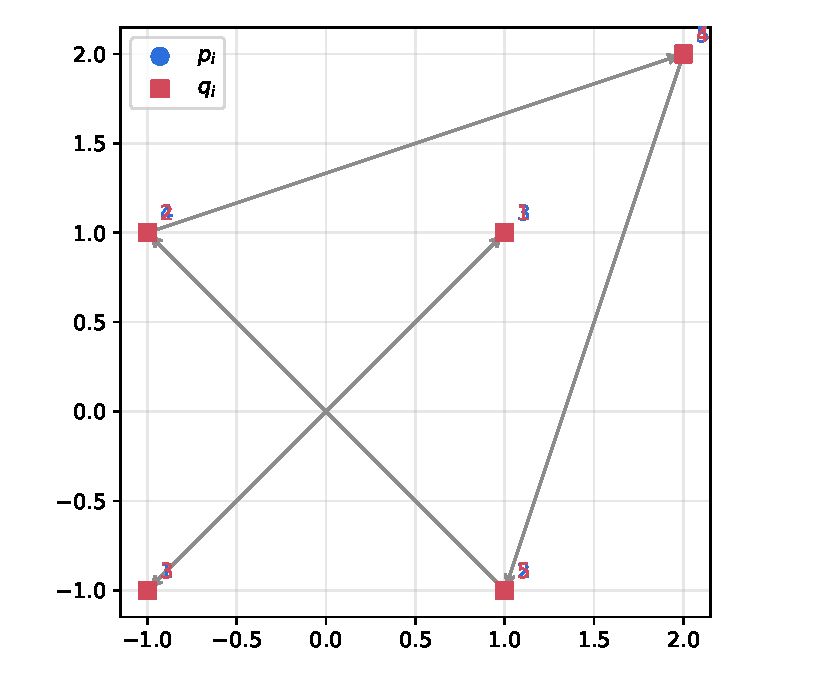
\includegraphics[width=0.55\textwidth]{gen/bijekcja.pdf}\caption{Zadana bijekcja $p_i\mapsto q_i$.}\end{figure}}{}